\section{Application}
	\subsection{Réception superhétérodyne}
		un réception superhétérodyne est un récepteur conçu sur le principe de mélange de fréquences. Permet de convertir le signal reçu en une fréquence intermédiaire plus basse qui est plus facile a utiliser. Avec une fréquence plus faible, ils est plus facile d'amplifier et de démoduler.
	
		\begin{equation}
			 f_{IF} = f_{rx}-f_{local}
		\end{equation}
		\begin{equation}
			 f_{IF} = f_{local}-f_{rx}
		\end{equation}
		
		les 2 fréquence sont symétriques autour de $f_{local}$ et on récupère (13) qui est la fréquence plus basse du signal recu via un filtre passe-bas
		
	\subsection{Radio}
		\subsubsection{Pouquoi plus radio FM que AM ?}
			\begin{itemize}
				\item \textbf{AM :} entre 600 et 900 kHz donc = 300kHz donc $\cfrac{300kHz}{30kHz} \approx 10$ donc asser de place pour 10 chaines de radio
				\item \textbf{FM :} entre 85 et 105 MHz donc 23MHz donc $\cfrac{23 000 MHz}{30kHz} \approx 766$ donc asser de place pour 766 chaines de radio
			\end{itemize}
			
		\subsection{Signal stéréo Radio}
			C'est la composition de plusieurs signaux formant un signal composite :
			\begin{itemize}
				\item G+D signal mono
				\item G-D signal supplémentaire pour crée le stéréo
			\end{itemize}
		
			\subsubsection{Modulation}
				
				Création du signal composite dans une bande FM:
				
				Un signal mono (G+D) + un modulation AM contenant a la fois G+D et G-D + pilote = porteuse de 30kHZ divisé par 2 sinon interférence avec le signal G-D
				
				\begin{figure}[htp]
				\centering
				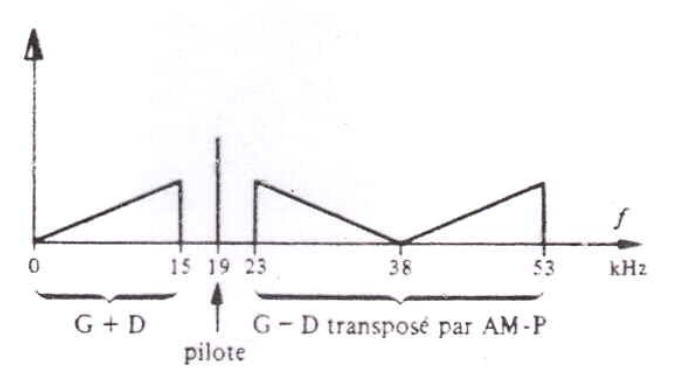
\includegraphics[width=0.6\textwidth]{img/signalStéréo.png}
				\end{figure}
			
			\subsubsection{Emetteur}
				Permet la création du signal stéréo
				
				\begin{enumerate}
					\item on a 2 signaux $x_L$ et $x_R$ pour gauche et droite
					\item on va former $x_L + x_R$ (G+D) et $x_L - x_R$
					\item on crée un sinusoîde localement a 38 kHz
					\item on la multiplie avec $x_L - x_R$ pour former G-D transposé comme sur la figure au dessus
					\item on divise par 2 la fréquence de la sinusoïde pour crée le pilote de 19 kHz
					\item on additione $x_L + x_R$, $x_L - x_R$ et le pilote et la somme vont former le signal composite qui est envoyé par le modulateur
				\end{enumerate}
				
				\begin{figure}[htp]
				\centering
				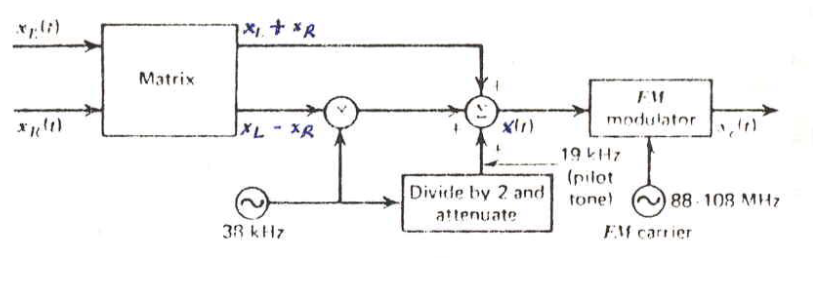
\includegraphics[width=0.6\textwidth]{img/emeteurStereo.png}
				\end{figure}
				
			\subsubsection{Récepteur stéréo }
				
				Permet la réception du signal mono ou stéréo
				
				\begin{enumerate}
					\item Effectue une démodulation FM pour récupéré le signal composite
					\item récupere G+D\\
						(a) utilise un filtre passe-bas 15 kHz (c'est la seul donnée nécessaire pour le MONO)
						
					\item recupere le pilote\\
						(a) utilise un filtre passe-bande 19kHz\\
						(b) multiplication de la fréquence du pilote par 2  pour crée porteuse de 38 kHz
					\item récupère G-D transposé \\
						(a) utilise un filtre passe-bande entre 23kHz et 53kHz
					\item démodulation du signal G-D transposé avec la porteuse de 38kHz (centre le signal autour de 0)
					\item utilise un filtre passe-bas de 15 kHz pour récuperer le signal original G-D
					\item Recombinaison des signaux G-D G+D pour crée le signal stéréo
				\end{enumerate}
				
				\begin{figure}[htp]
				\centering
				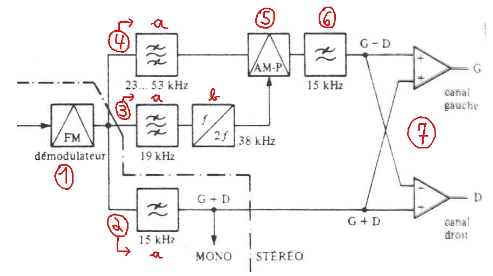
\includegraphics[width=0.6\textwidth]{img/recepteurStereo.png}
				\end{figure}
		\subsection{TV noir et blanc}
			\subsubsection{Modulation}
				 Création d'un signal composite contenant
				 \begin{itemize}
				 	\item signal vidéo (porteuse a $\approx$ 4 MHz)
				 	\item signal audio (porteuse a $\approx$ 4.5 MHZ) modulé en FM
				 	
				 \end{itemize}
				 
				 \begin{figure}[htp]
				\centering
				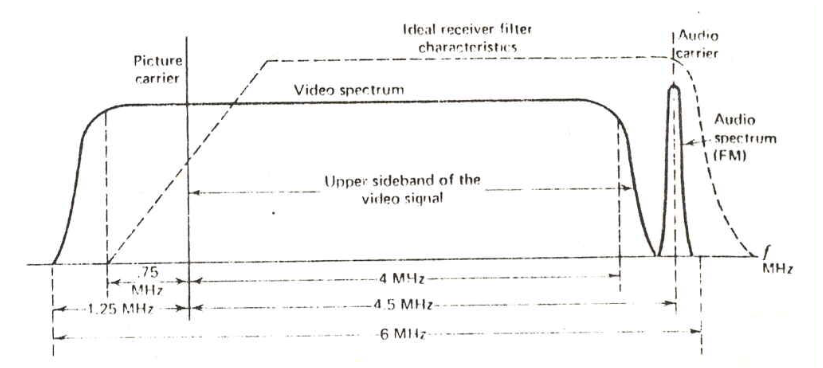
\includegraphics[width=0.7\textwidth]{img/ModulationTVNoirBlanc.png}
				\end{figure}
			\subsubsection{Emetteur}
				\textbf{Audio} : 
				\begin{enumerate}
					\item Recupere le signal audio grace au micro
					\item utilise le modulateur de fréquence audio 4.5 MHz (audio carrier) pour faire une modulation FM du signal audio\\
					
				\textbf{Vidéo} : \\
					\item Récupere signal audio par la caméra
					\item Utilise modulateur de fréquence vidéo (vidéo carrier) pour faire modulation AM du signal vidéo\\
					
				\textbf{Final} :\\
				
				\item additionner signal audio et vidéo
				\item modulation du resultat des signaux (VSB filter)
				\end{enumerate}
				
				\begin{figure}[htp]
				\centering
				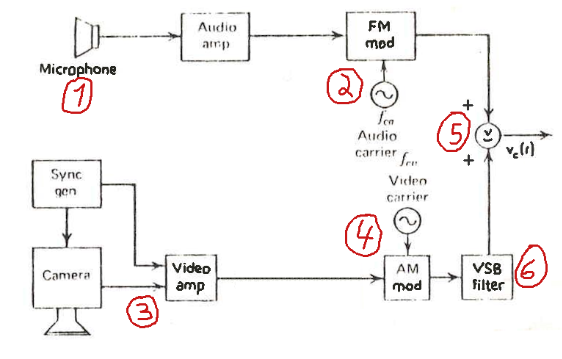
\includegraphics[width=0.7\textwidth]{img/EmetteruTVNoirBlanc.png}
				\end{figure}
				
			\subsubsection{Recepteur}
				Permet réception signal TV noir et blanc
				\begin{enumerate}
					\item récupération signal par antenne
					\item Démodulation pour arriver a une fréquence intermédiaire
					\item Démodulation FM pour récupérer signal audio
					\item Démodulation AM pour récupérer signal vidéo
					
				\end{enumerate}
				
				\begin{figure}[htp]
				\centering
				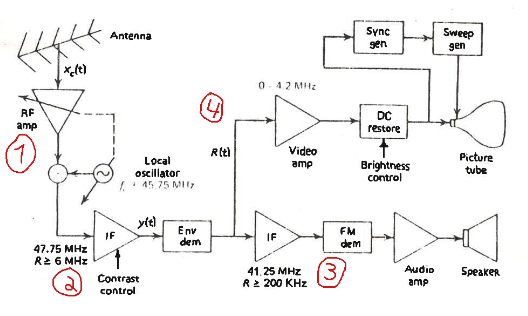
\includegraphics[width=0.7\textwidth]{img/recepteurTVNoirBlanc.png}
				\end{figure}
		\newpage
		\subsection{TV couleurs}
			\textcolor{red}{R} \textcolor{green}{G} \textcolor{blue}{B} $\Rightarrow$ Y U V
			
			Y = 0.30 \textcolor{red}{R} + 0.59 \textcolor{green}{G} + 0.11\textcolor{blue}{B}
			
			U = 0.493 (\textcolor{blue}{B} - Y)
			V = 0.877 (\textcolor{red}{R} - Y)
			
			Y = luminance $\Rightarrow$ signal de noir et blanc
			U et V = Chrominances $\Rightarrow$ Signaux pour récupéré les info de couleurs
			
			On envois 3 signaux de couleur R G B pour pouvoir continuer a utilise les tv en noir et blanc (Y)
			
			\subsubsection{Système NTSC}
				Luminance : VSB
				
				Chrominances : QAM
				
				Son : FM
				
				\begin{figure}[htp]
				\centering
				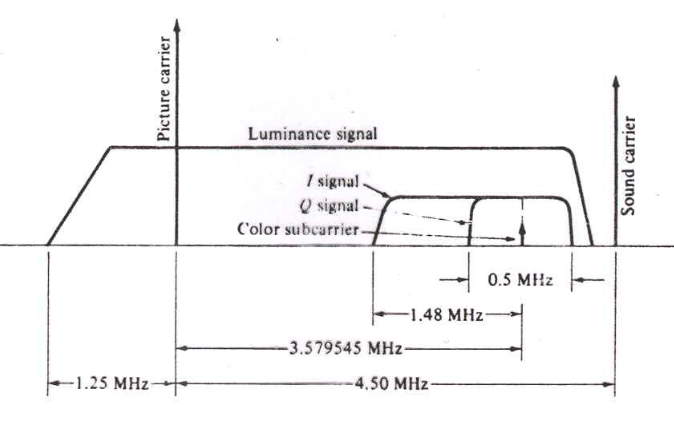
\includegraphics[width=0.6\textwidth]{img/NTSC.png}
				\end{figure}
			\subsubsection{Système PAL}
				Facilite la démodulation QAM des chrominances
				\begin{equation}
					v(t) = U\sin (\omega_c t) \theta \pm V \cos (\omega_c t)
				\end{equation}
				
				Le $\pm$ fait tous, $\Rightarrow$ "Phase alternating line" : Plus de tolérance pour les erreurs de phase
				
				\begin{itemize}
					\item U et V avec la meme largueur de bande
					\item Spectre (contenue fréquentiel) plus compliqué
					\item Porteuse plus éloignée
				\end{itemize}
				
				\begin{figure}[htp]
				\centering
				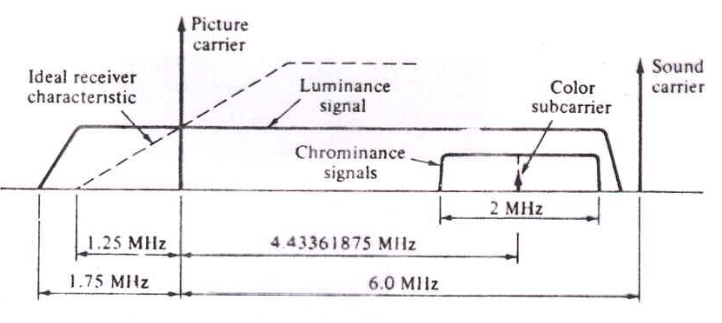
\includegraphics[width=0.7\textwidth]{img/PAL.png}
				\end{figure}
				
			\subsubsection{Création du signal PAL}
			
			\begin{figure}[htp]
				\centering
				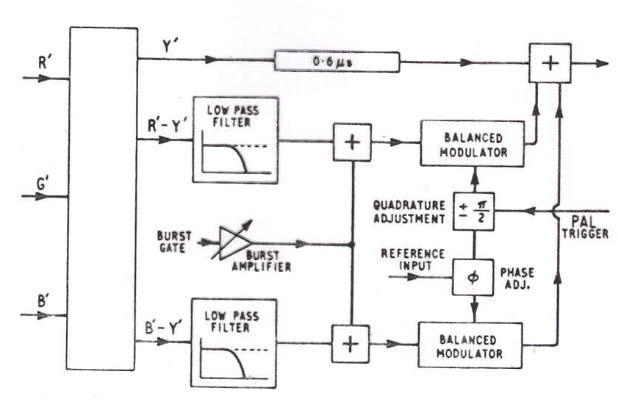
\includegraphics[width=0.7\textwidth]{img/PAL1.png}
			\end{figure}
				
				
			\subsubsection{Systheme SECAM}
				"Séquentiel a mémoire"
				
				On ne transmet chaque chrominance qu'une ligne sur 2 et on les moduel en FM pour eviter les difficulté de la QAM
				
		\subsection{TV numérique}
			y = 0.299 \textcolor{red}{r} + 0.587 \textcolor{green}{g} + 0.114 \textcolor{blue}{b}
			
			Y = 219 y + 16
			
			CR = $\cfrac{112(\textcolor{red}{r} - y)}{0.701} + 128$
			
			CB = $\cfrac{112(\textcolor{blue}{b} - y)}{0.886} + 128$
			
			
			La luminance : Y echantillonné a 13.5MHz (864 ech/ligne)
			13.5MHz car :
			\begin{itemize}
				\item Theoreme de Shannon ($f_{ech} > 2 f_{MAX}$)
				\item On travaille sur une bande de max 6MHz cf Systeme PAL
				\item Le signal vidéo a donc une fréquence de 6MHz
				\item La fréquene d'echantillionnage doit etre plus grande que 12MHZ ($f_{ech} > 12MHz$)
			\end{itemize}
			
			CR et CB (signaux de chrominance) sont echnatiollonées a 6.75 MHZ (432 ech/ligne)
			
			Quantification 8 bits/echantillions $\Rightarrow$ 216Mbs avant compression
			
			\textbf{Avantages}:
			\begin{itemize}
				\item compression
				\item Code correcteur erreurs + "regénérations"
				\item Qualité optimale dès que la transmission est assez bonne
				\item Permet de transmettre + de cannaux dans la même bande
				\item Possibilités d’enregistrements, etc \dots 
			\end{itemize}
			
			\textbf{Désavantages}
			\begin{itemize}
				\item Délais de zapping (codage)
				\item Dégradation rapide si mauvais signal
			\end{itemize}